\section{Synthetic experiments and results}
\label{sec:experiments}

\subsection{Synthetic arrivals and comparison protocol}
\label{subsec:synthetic_data}

Synthetic first-arrival times are generated independently of EMTomo using PyKonal 0.4.1 \parencite{white2020pykonal}. The generator solves the Cartesian eikonal equation from the true event coordinates on a refined nodal grid, initializes off-grid sources with local straight-segment slowness integrals, and samples receivers by interpolating the regular factor $T(\mathbf{x})/\|\mathbf{x}-\mathbf{h}\|$. For the v1.4 layered runs, this differs from EMTomo's station-centered \texttt{scikit-fmm} fields, homogeneous source-sphere initialization, and direct interpolation of travel times. Separate solvers, grids, and source treatments reduce numerical inverse crime; both still approximate the same isotropic first-arrival problem, so this is not a test against independent wave physics.

Before referencing each event to its earliest observed arrival, we add independent Gaussian errors
\begin{equation}
t^{\mathrm{noisy}}_{en}=T^{\mathrm{true}}_{en}
+0.01T^{\mathrm{true}}_{en}Z^{(1)}_{en}+\sigma_a Z^{(2)}_{en},
\qquad Z^{(1)}_{en},Z^{(2)}_{en}\sim\mathcal{N}(0,1),
\end{equation}
with $\sigma_a=0.05$~s for the checkerboards and $0.01$~s for the layered models, using seed 42. Thus the pre-reference noise variance is $(0.01T^{\mathrm{true}}_{en})^2+\sigma_a^2$, not the square of a sum of standard deviations. All event--station pairs are observed. EMTomo and tomoDD use the same saved picks within each experiment, but only tomoDD receives an initial hypocenter catalog. In what follows, a \emph{zero-noise start} means true initial hypocenters for tomoDD, not noise-free arrival times. Inter-event differential times for tomoDD are formed from these picks; no additional waveform cross-correlation observations are supplied.

The methods retain their native velocity representations and regularization. Their iteration counts are not equated: the checkerboards use 12 EMTomo updates and three tomoDD iterations; the layered tests use eight or 12 EMTomo updates and three tomoDD iterations. We evaluate the specified checkpoints, including iteration three of a tomoDD run that continued further, rather than silently substituting its final model. These are comparisons of the stated workflows, not controlled tests differing only in location-uncertainty treatment. A single noise seed is used; the results do not establish statistical superiority across realizations.

\subsection{Quality metrics and representation oracles}
\label{subsec:metrics}

\paragraph{Velocity fields.}
We evaluate the native reconstructed fields at the same physical points $\{\mathbf{x}_q\}_{q=1}^Q$, without converting one method to the other's parameterization. EMTomo is piecewise constant; tomoDD is evaluated by its native trilinear velocity interpolation, including the fixed exterior nodes. The principal measures are
\begin{equation}
\mathrm{RMSE}_v=\sqrt{\frac{1}{Q}\sum_q[\widehat v(\mathbf{x}_q)-v^{\mathrm{true}}(\mathbf{x}_q)]^2},
\qquad
\mathrm{MAE}_v=\frac{1}{Q}\sum_q|\widehat v(\mathbf{x}_q)-v^{\mathrm{true}}(\mathbf{x}_q)|.
\label{eq:velocity_metrics}
\end{equation}
Whole-volume scores are accompanied by regional scores: interfaces versus block interiors for checkerboards, and individual spheres versus the surrounding medium for layered models. Native coarse-grid quality logs and travel-time residuals are not interchangeable with these field errors.

\paragraph{Hypocenters.}
For hard EMTomo and tomoDD, define $d_e=\|\widehat{\mathbf{h}}_e-\mathbf{h}^{\mathrm{true}}_e\|$. We report the catalog RMS $\sqrt{E^{-1}\sum_e d_e^2}$, median, and 95th percentile, with coordinate biases as diagnostics. For soft EMTomo we use the largest-weight hypothesis for the same point-location comparison and additionally score the entire discrete distribution. Probabilistic location methods distinguish optimal locations from their uncertainty \parencite{lomax2000,smith2022}; to evaluate our weighted hypotheses without imposing a Gaussian shape or an arbitrary smoothing bandwidth, we choose the energy score \parencite{gneiting2007}:
\begin{equation}
\mathrm{ES}_e=\sum_j w_{ej}\|\mathbf{h}_{ej}-\mathbf{h}^{\mathrm{true}}_e\|
-\frac{1}{2}\sum_{j,k}w_{ej}w_{ek}\|\mathbf{h}_{ej}-\mathbf{h}_{ek}\|.
\label{eq:energy_score}
\end{equation}
Lower mean ES is better; for a single hypothesis it equals the mean location distance, not the RMS. This proper score assesses probabilistic accuracy, but a low score alone does not demonstrate calibrated credible regions. We also retain the weighted-mean location error and the spread around that mean; averaging separated modes can place the mean in an implausible location, so it does not replace the mode-based comparison.

All events receive equal weight in catalog statistics. The available EMTomo locations belong to the E-step immediately preceding the selected last velocity update, whereas velocity scores use the post-update model. They are explicitly labeled as such, not presented as a final relocation in that updated model. A final location-only pass is needed for fully synchronized velocity--hypocenter checkpoints.

\paragraph{Spherical anomalies.}
Let $v_b$ denote the known layered background and $\delta v^{\mathrm{true}}=v^{\mathrm{true}}-v_b$. In addition to RMSE on the nonzero support $S_k$ of each sphere, we measure its signed template-amplitude recovery:
\begin{equation}
a_k=\frac{\sum_{\mathbf{x}_q\in S_k}
[\widehat v(\mathbf{x}_q)-v_b(\mathbf{x}_q)]\,\delta v^{\mathrm{true}}(\mathbf{x}_q)}{
\sum_{\mathbf{x}_q\in S_k}[\delta v^{\mathrm{true}}(\mathbf{x}_q)]^2}.
\label{eq:sphere_amplitude}
\end{equation}
For an otherwise correct background, $a_k=0$ means absent contrast, $a_k=1$ the true template amplitude, and $a_k<0$ reversed contrast. This is a projection onto the true anomaly, not a peak-velocity ratio: displacement, shape distortion, and background errors also affect it. RMSE inside the sphere and outside all spheres distinguishes contrast recovery from local error and degradation of the background. No thresholded sphere segmentation is needed.

\paragraph{Oracles.}
For each representation, a truth-only oracle fits velocity values to the known field, without using arrivals or estimating hypocenters. For constant cells, the volume squared-error optimum is the arithmetic mean of true velocity within each cell, \emph{not} the inverse of mean slowness. For tomoDD we use the saved least-squares trilinear truth fit with the same free nodes and fixed exterior values as the inversion. These references quantify representational error, not the resolution attainable from the available rays, and are distinct from an inversion with fixed true hypocenters. A whole-volume oracle is not a lower bound for every regional RMSE, and the difference between reconstruction and oracle RMSE is not an additive decomposition of inversion error.

The checkerboard truth is exactly representable by EMTomo's aligned constant cells, so its oracle is the true field. This is \emph{not} true for the layered sphere models on the coarser inversion grid: they require a separate cell-mean oracle. Because the two layered experiments share the same truth and grids, they share both representation oracles and initial native fields.

\subsection{Checkerboards with varying anomaly size}
\label{subsec:checkerboard_results}

The first series occupies $240\times120\times120$~km. Alternating cubes have velocities 4750 and 5250~m/s and sides 60, 40, or 30~km (respectively $4\times2\times2$, $6\times3\times3$, or $8\times4\times4$ cubes). The same 1200 synthetic events and 98 surface stations are used in all cases. EMTomo has $24\times12\times12$ constant 10-km cells; tomoDD has 3456 free interior velocity nodes at the same centers, with fixed exterior faces. Both start at 5000~m/s. EMTomo uses one active location hypothesis, 12 updates, subdivision nine, damping parameter 0.05, and a $\pm0.5\%$ cellwise velocity-step limit. TomoDD uses three joint iterations, damping 150, smoothing 40/40/30, and initial hypocenters perturbed independently by 2~km standard deviation in each coordinate. Candidate initial coordinates outside the domain are rejection-resampled. Its event-pair graph uses a 30-km cutoff and maximum degree ten.

These saved checkerboard runs are labeled EMTomo v1.1 and predate the current unified likelihood and exact-coordinate station initialization. Their metadata does not preserve runtime source hashes; the archived pre-run source uses cell-center station seeding and an unweighted within-event pairwise residual, rather than the current precision-weighted formulation. We therefore treat this series as a legacy parameterization benchmark, not a validation of every implementation detail in Section~\ref{sec:method}.

All fields are scored at 432,000 common 2-km voxel centers. The initial-model RMSE is 250~m/s. Table~\ref{tab:checkerboards} reports the reconstruction and oracle errors. The saved trilinear oracles were fitted on the original runs' sampling grids and then evaluated at these common points; they are representation references, not guaranteed exact minima of the common-grid objective.

\begin{table}[tbp]
\centering
\caption{Checkerboard whole-volume velocity RMSE (m/s). EMTomo uses a single active location hypothesis. Its representation oracle has zero error in every case.}
\label{tab:checkerboards}
\begin{tabular}{rrrr}
\toprule
Cube side (km) & EMTomo & tomoDD & Trilinear oracle \\
\midrule
60 & 185.62 & 142.30 & 76.10 \\
40 & 166.15 & 169.33 & 97.24 \\
30 & 169.33 & 173.22 & 116.37 \\
\bottomrule
\end{tabular}
\end{table}

TomoDD has lower volume RMSE for 60-km cubes; for 40- and 30-km cubes the differences favoring EMTomo are only 3.18 and 3.89~m/s. EMTomo has lower error within 5~km of true internal block faces in all three cases, whereas tomoDD has lower error in block interiors. The increasing trilinear-oracle error with decreasing cube size illustrates why sharper block boundaries alone do not establish a resolution advantage (Figure~\ref{fig:checkerboards}). TomoDD's final hypocenter RMS is 1.774, 1.714, and 1.777~km, respectively, from the same 3.462-km initial RMS. EMTomo's corresponding location scores have not yet been extracted for this series.

\begin{figure}[tbp]
\centering
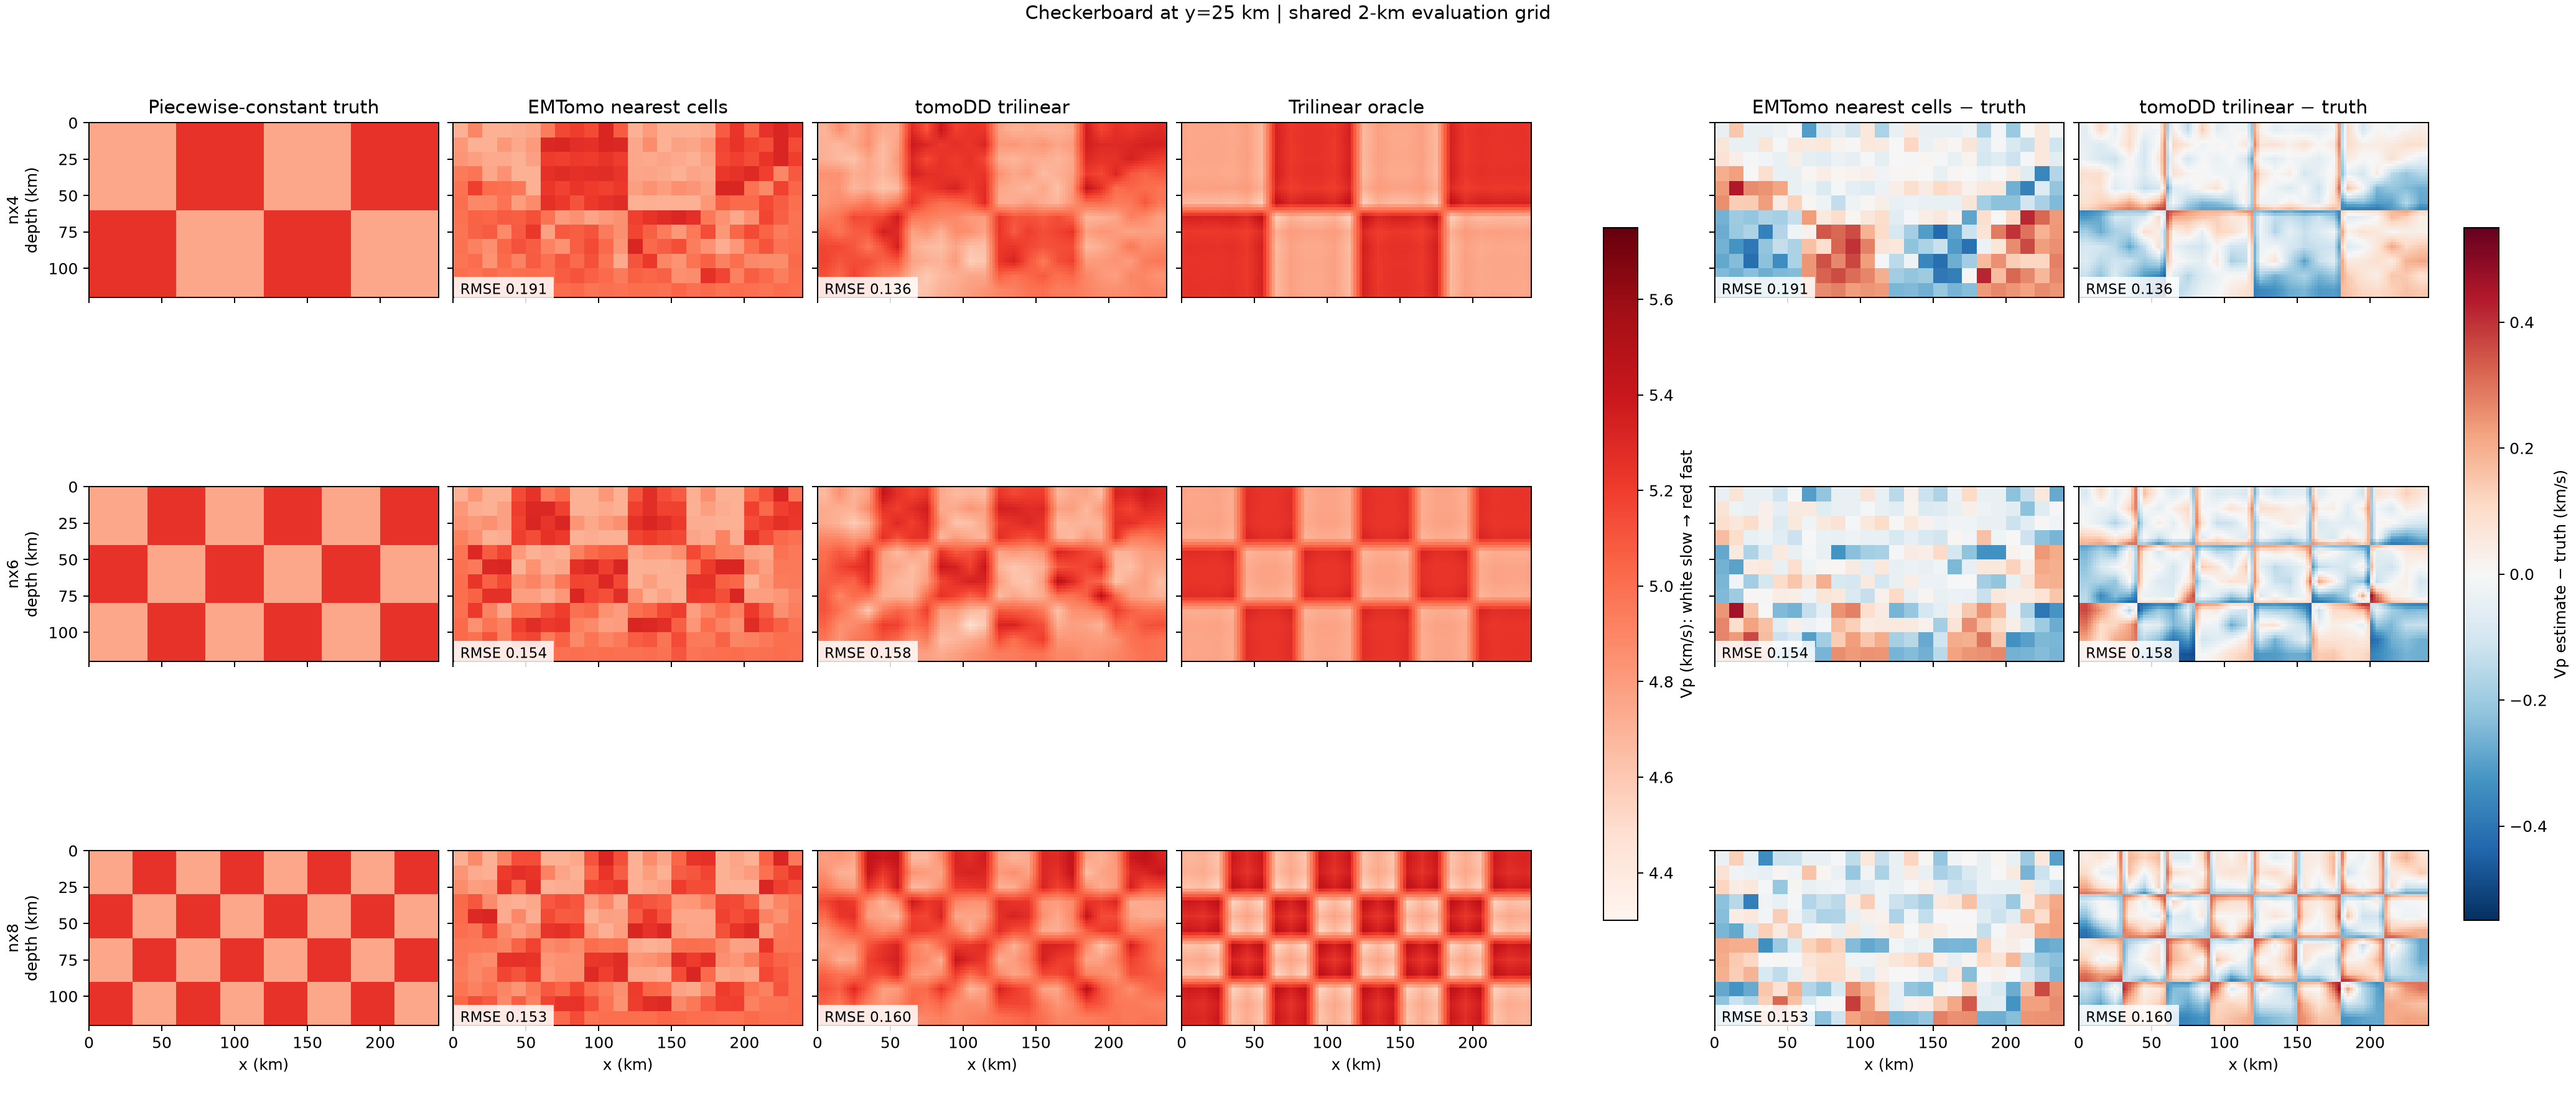
\includegraphics[width=\textwidth]{figures/checkerboard_y25km.png}
\caption{Checkerboard vertical section at $y=25$~km. Rows have cube sides 60, 40, and 30~km; columns show truth, EMTomo, tomoDD, the trilinear oracle, and the two reconstruction errors. Figure velocity and error scales are in km/s; table scores are in m/s. Slice RMSE is not the whole-volume RMSE.}
\label{fig:checkerboards}
\end{figure}

\subsubsection{Scaled checkerboards with the current implementation}
\label{subsec:scaled_checkerboards}

Figures~\ref{fig:checkerboard_geometry_current} and~\ref{fig:checkerboard_comparison_current} show a separate, scaled checkerboard series on a $24\times12\times12$~km domain, with cube sides 6, 4, and 3~km ($n_x=4,6,8$). The geometry contains 1200 events and 98 surface stations. Both methods start from a homogeneous 5~km/s velocity model and use 1-km velocity parameterizations. The saved observations in this series have 1\% relative and 0.01-s absolute pre-reference noise. EMTomo uses 12 hard-assignment updates, 15 candidates with top-1 selection, regularization parameter $\lambda=1$, and coverage-damping power zero. The tomoDD results are from three joint iterations with a 1-km per-coordinate Gaussian perturbation of the initial hypocenters (seed 42). The numerical scores in Table~\ref{tab:checkerboards} describe the legacy, larger-domain runs above, not these scaled reconstructions.

\clearpage
\begin{landscape}
\begin{figure}[p]
\centering
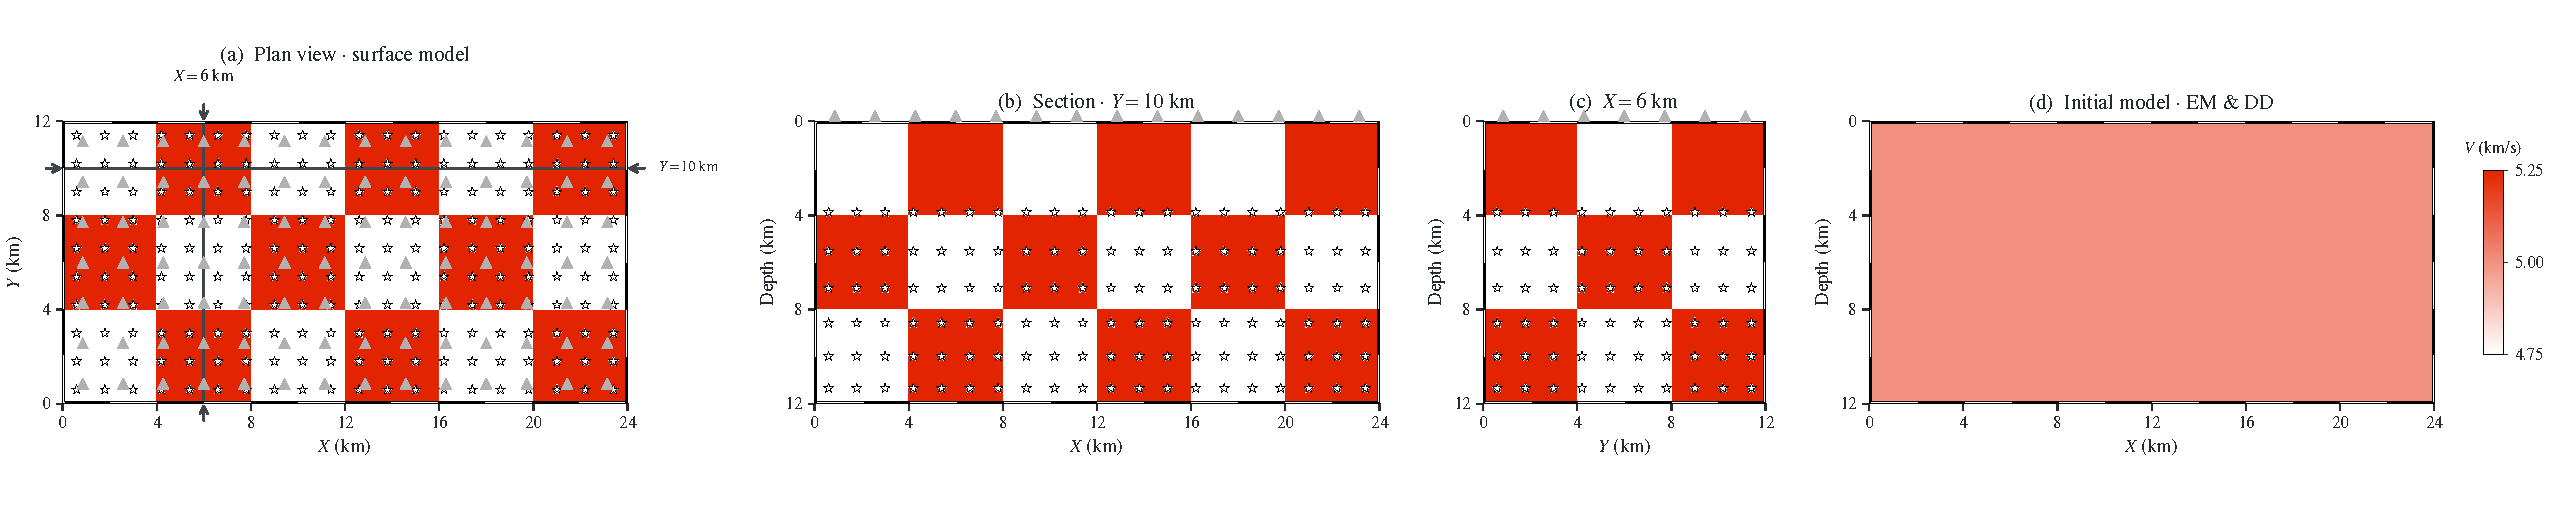
\includegraphics[width=\linewidth]{figures/checkerboard_nx6_geometry.pdf}
\begin{singlespace}
\caption{Scaled checkerboard model and acquisition geometry for $n_x=6$. (a) Surface velocity field and plan-view projections of stations (grey triangles) and events (white stars); arrows mark the sections at $Y=10$~km and $X=6$~km. (b,c) The corresponding vertical velocity sections, with all stations and events projected onto each plane. Coincident projections are drawn once: each event marker represents six events in (a), ten in (b), and twenty in (c); station markers represent seven stations in (b) and fourteen in (c). (d) The common homogeneous initial velocity model for EMTomo and tomoDD, also used for $n_x=4$ and 8. Depth is positive downward. Alternating frame segments are 2~km long.}
\label{fig:checkerboard_geometry_current}
\end{singlespace}
\end{figure}
\end{landscape}

\begin{figure}[p]
\centering
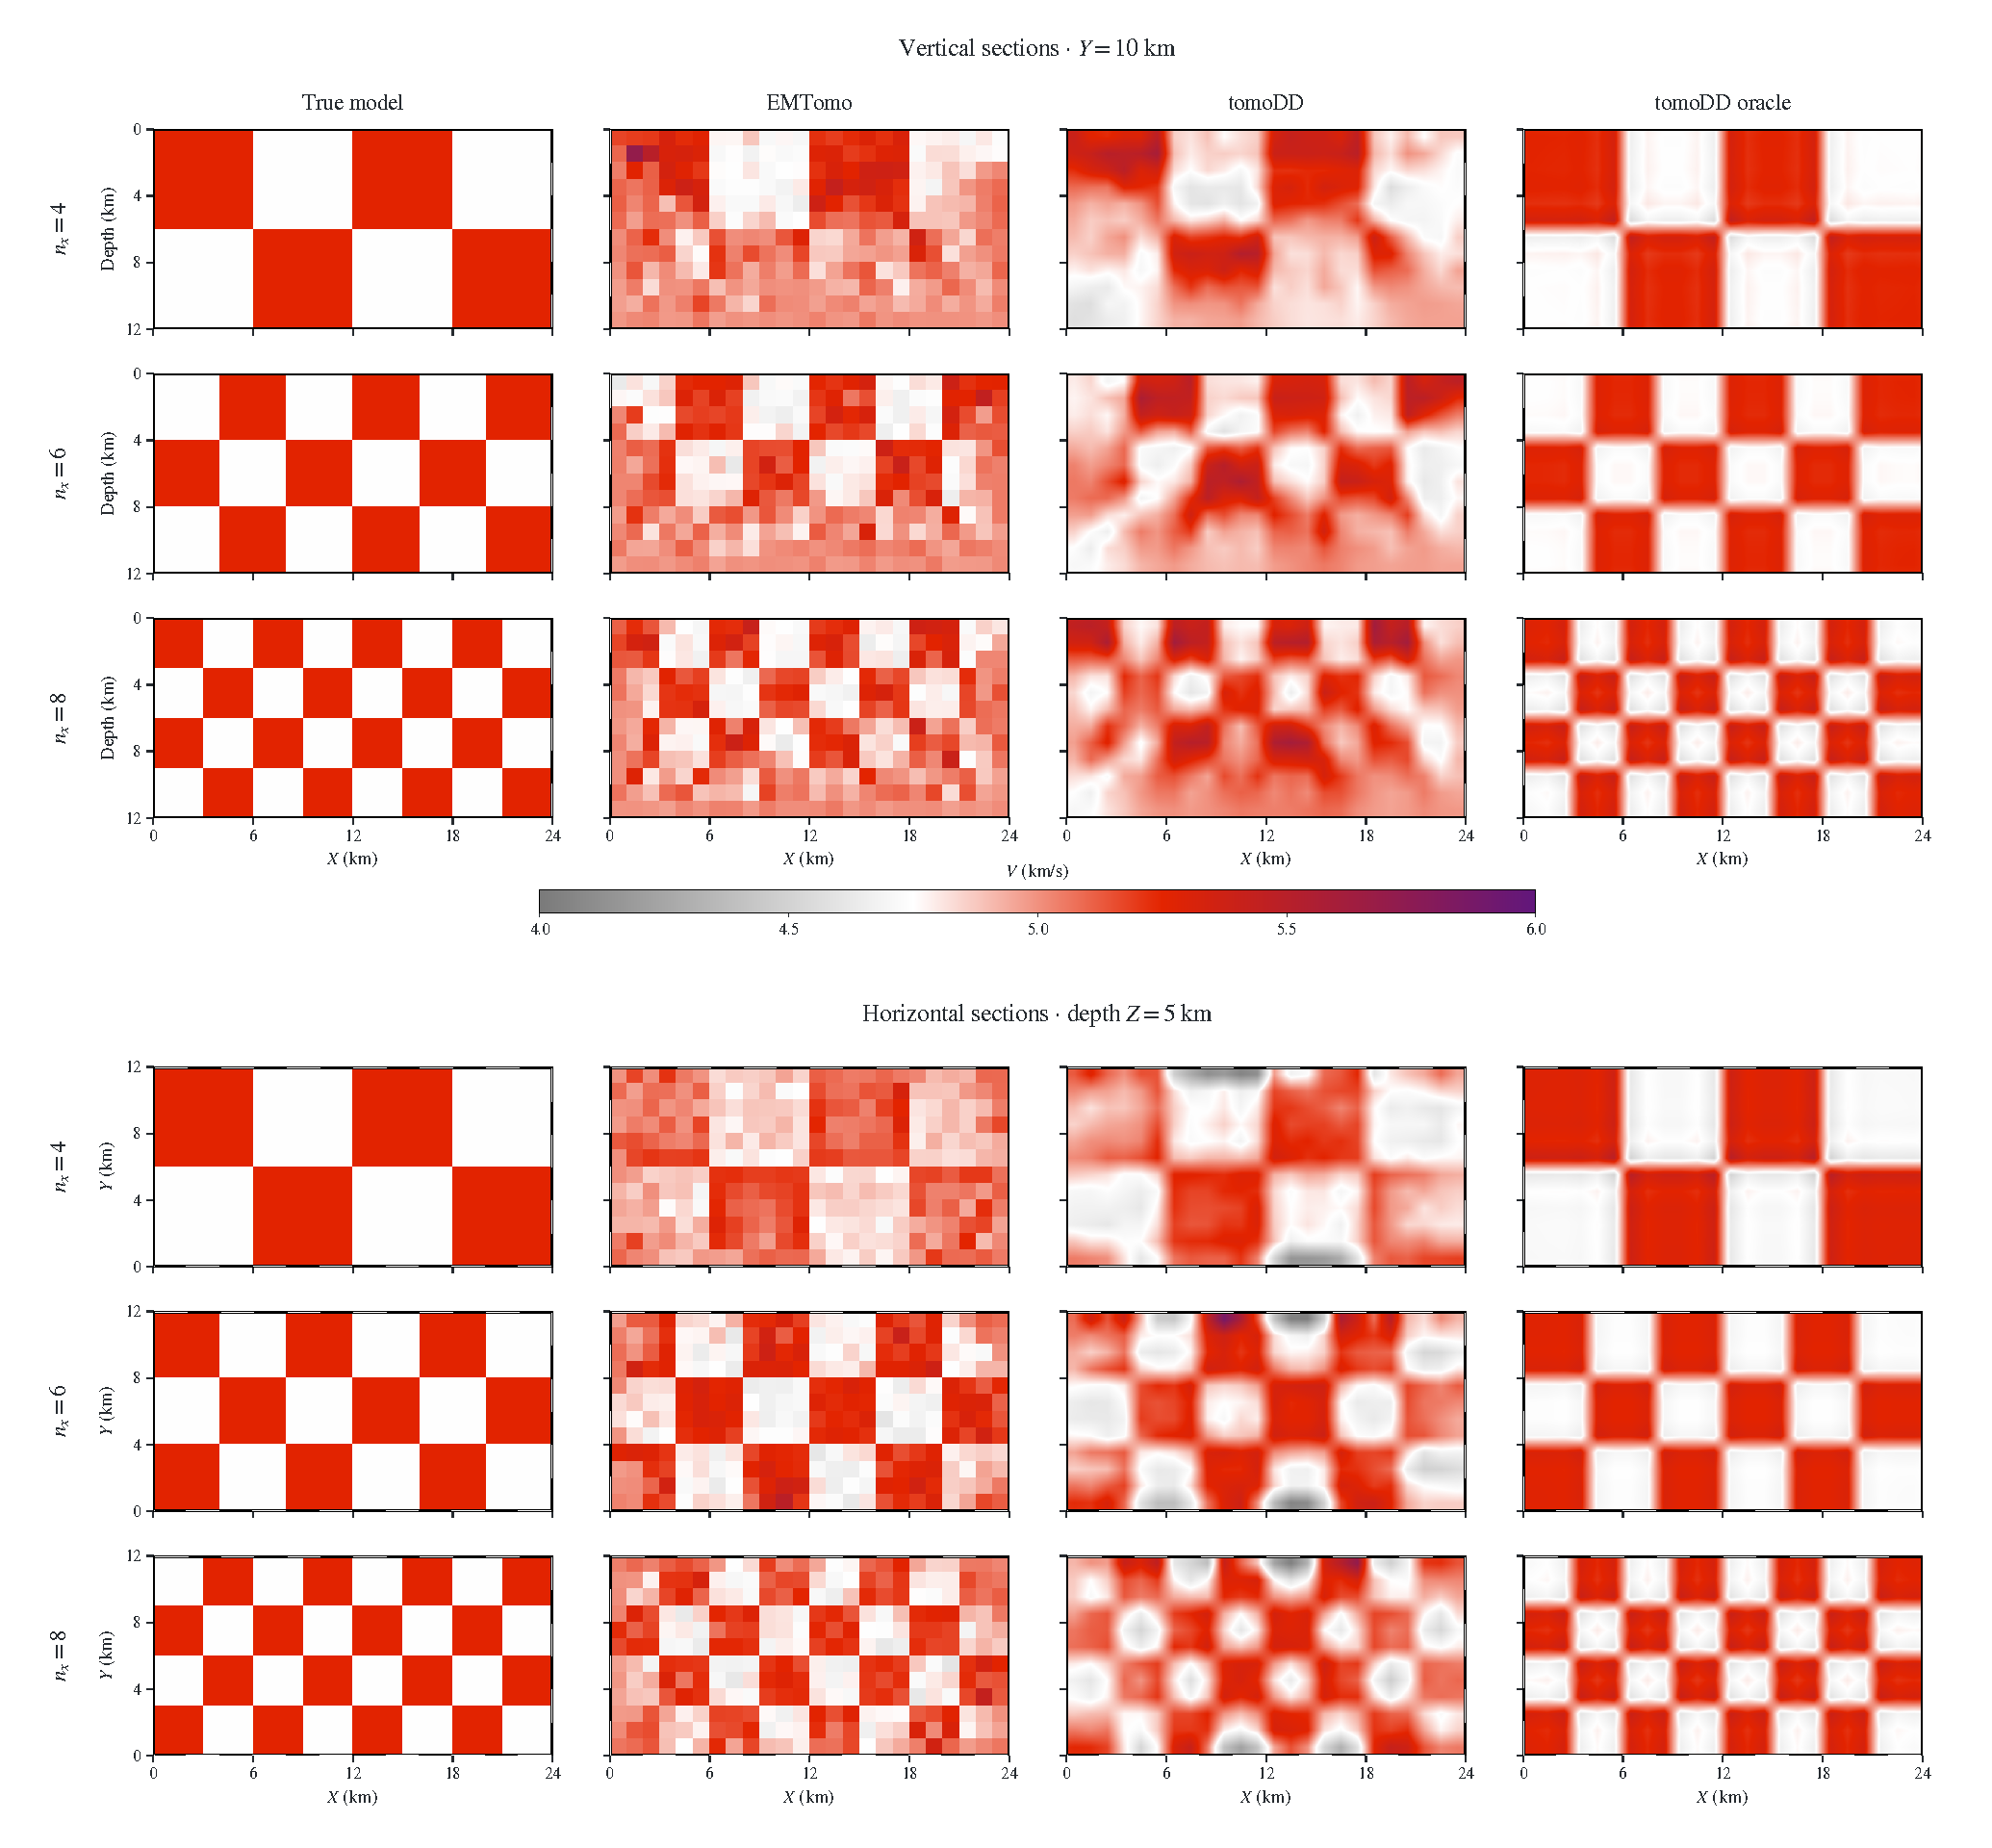
\includegraphics[width=\textwidth,height=0.79\textheight,keepaspectratio]{figures/checkerboard_nx4_nx6_nx8_comparison.pdf}
\begin{singlespace}
\caption{Scaled checkerboard reconstructions. Columns show truth, EMTomo after 12 updates with coverage-damping power zero, tomoDD after three iterations, and the saved trilinear representation oracle. The upper three rows are vertical sections at $Y=10$~km for $n_x=4,6,8$; the lower three rows are horizontal sections at depth $Z=5$~km in the same order. True and EMTomo fields are piecewise constant; tomoDD and its oracle use native trilinear velocity interpolation. The oracle is a truth-only representation reference, not an inversion result. All panels share the velocity scale in km/s; no stations or events are overlaid.}
\label{fig:checkerboard_comparison_current}
\end{singlespace}
\end{figure}
\clearpage

\subsection{Layered model with spherical anomalies: artificial geometry}
\label{subsec:sphere_results}

The second series uses a $20\times7\times7$~km model sampled on 125-m truth cells. Four horizontal layers have velocities 3800, 4600, 5200, and 5700~m/s, with interfaces at 0.7, 1.9, and 3.4~km. Six additive spherical anomalies are specified in Table~\ref{tab:sphere_truth}. Each has constant peak contrast inside half its radius and a cosine taper to zero at its outer radius. The starting model contains only the layers. Since the interfaces do not align with 1-km inversion cells, the starting layered field itself has representation error.

\begin{table}[tbp]
\centering
\caption{Spherical anomalies shared by the artificial- and Geysers-geometry experiments. Coordinates and radii are in km; peak contrast is in m/s. Depth is positive downward.}
\label{tab:sphere_truth}
\begin{tabular}{rrrrrr}
\toprule
Sphere & $x$ & $y$ & $z$ & Radius & Peak $\delta v$ \\
\midrule
1 & 3.5 & 2.5 & 1.2 & 0.9 & $+600$ \\
2 & 8.0 & 4.8 & 2.0 & 1.1 & $-650$ \\
3 & 12.5 & 2.4 & 2.6 & 1.2 & $+700$ \\
4 & 16.5 & 4.5 & 1.6 & 1.0 & $-600$ \\
5 & 6.0 & 2.2 & 3.6 & 1.1 & $+700$ \\
6 & 11.0 & 5.0 & 4.0 & 1.0 & $-650$ \\
\bottomrule
\end{tabular}
\end{table}

There are 1920 events on a $24\times8\times10$ lattice, with actual depths 0.75--5.25~km, and 52 stations on a $13\times4$ surface grid. EMTomo uses 980 constant 1-km cells, subdivision eight, and hard assignment after refining five candidate cells per event. We score its eight-update checkpoint (damping 0.5, coverage-damping exponent one, velocity-step limit $\pm2\%$). TomoDD uses 980 free interior nodes with fixed padding, damping 40, smoothing 5/5/5, and a 0.05-km ray-derivative step. Its starts are either true hypocenters or locations perturbed by 0.5~km per coordinate; both are scored after three joint iterations. Their event-pair graphs use a 3-km cutoff and maximum degree four. No matched soft-EMTomo result is available yet for this geometry.

The common evaluation grid contains all 501,760 truth-cell centers. Only 15,314 centers belong to nonzero sphere support, so whole-volume error is dominated by the layered background. In the artificial geometry, EMTomo reduces volume RMSE from 215.43 to 202.86~m/s. Both tomoDD reconstructions recover the spheres more accurately in RMSE but have greater whole-volume error than their own trilinear starting field (Table~\ref{tab:flat4_velocity}). In this realization, a true initial catalog does not give the lowest tomoDD error. This cannot be attributed solely to initial-location accuracy: perturbing the catalog also changes the event-pair graph. Figure~\ref{fig:flat4_synthetic} shows the same physical section for the reconstructions, native initial models, and oracles.

\begin{table}[tbp]
\centering
\caption{Layered-model velocity RMSE (m/s), scored on the same 125-m truth grid. Zero and noisy tomoDD starts refer to initial hypocenters, not picks. The native initial fields and oracles are shared by both geometries. Regional oracle errors are descriptive, not regional lower bounds.}
\label{tab:flat4_velocity}
\small
\begin{tabular}{llrrr}
\toprule
Geometry & Model & Volume & Spheres & Outside spheres \\
\midrule
Artificial & EMTomo hard, 8 updates & 202.86 & 327.62 & 197.66 \\
 & tomoDD, zero start & 251.62 & 287.36 & 250.41 \\
 & tomoDD, noisy start & 208.12 & 273.49 & 205.72 \\
\midrule
Geysers & EMTomo hard, 12 updates & 208.32 & 329.69 & 203.32 \\
 & tomoDD, zero start & 188.75 & 276.76 & 185.30 \\
 & tomoDD, noisy start & 214.69 & 281.31 & 212.25 \\
\midrule
Both & EMTomo initial field & 215.43 & 427.24 & 205.24 \\
 & tomoDD initial field & 173.25 & 406.87 & 160.46 \\
 & Constant-cell oracle & 181.49 & 298.06 & 176.58 \\
 & Trilinear oracle & 142.86 & 233.91 & 139.03 \\
\bottomrule
\end{tabular}
\end{table}

\begin{figure}[tbp]
\centering
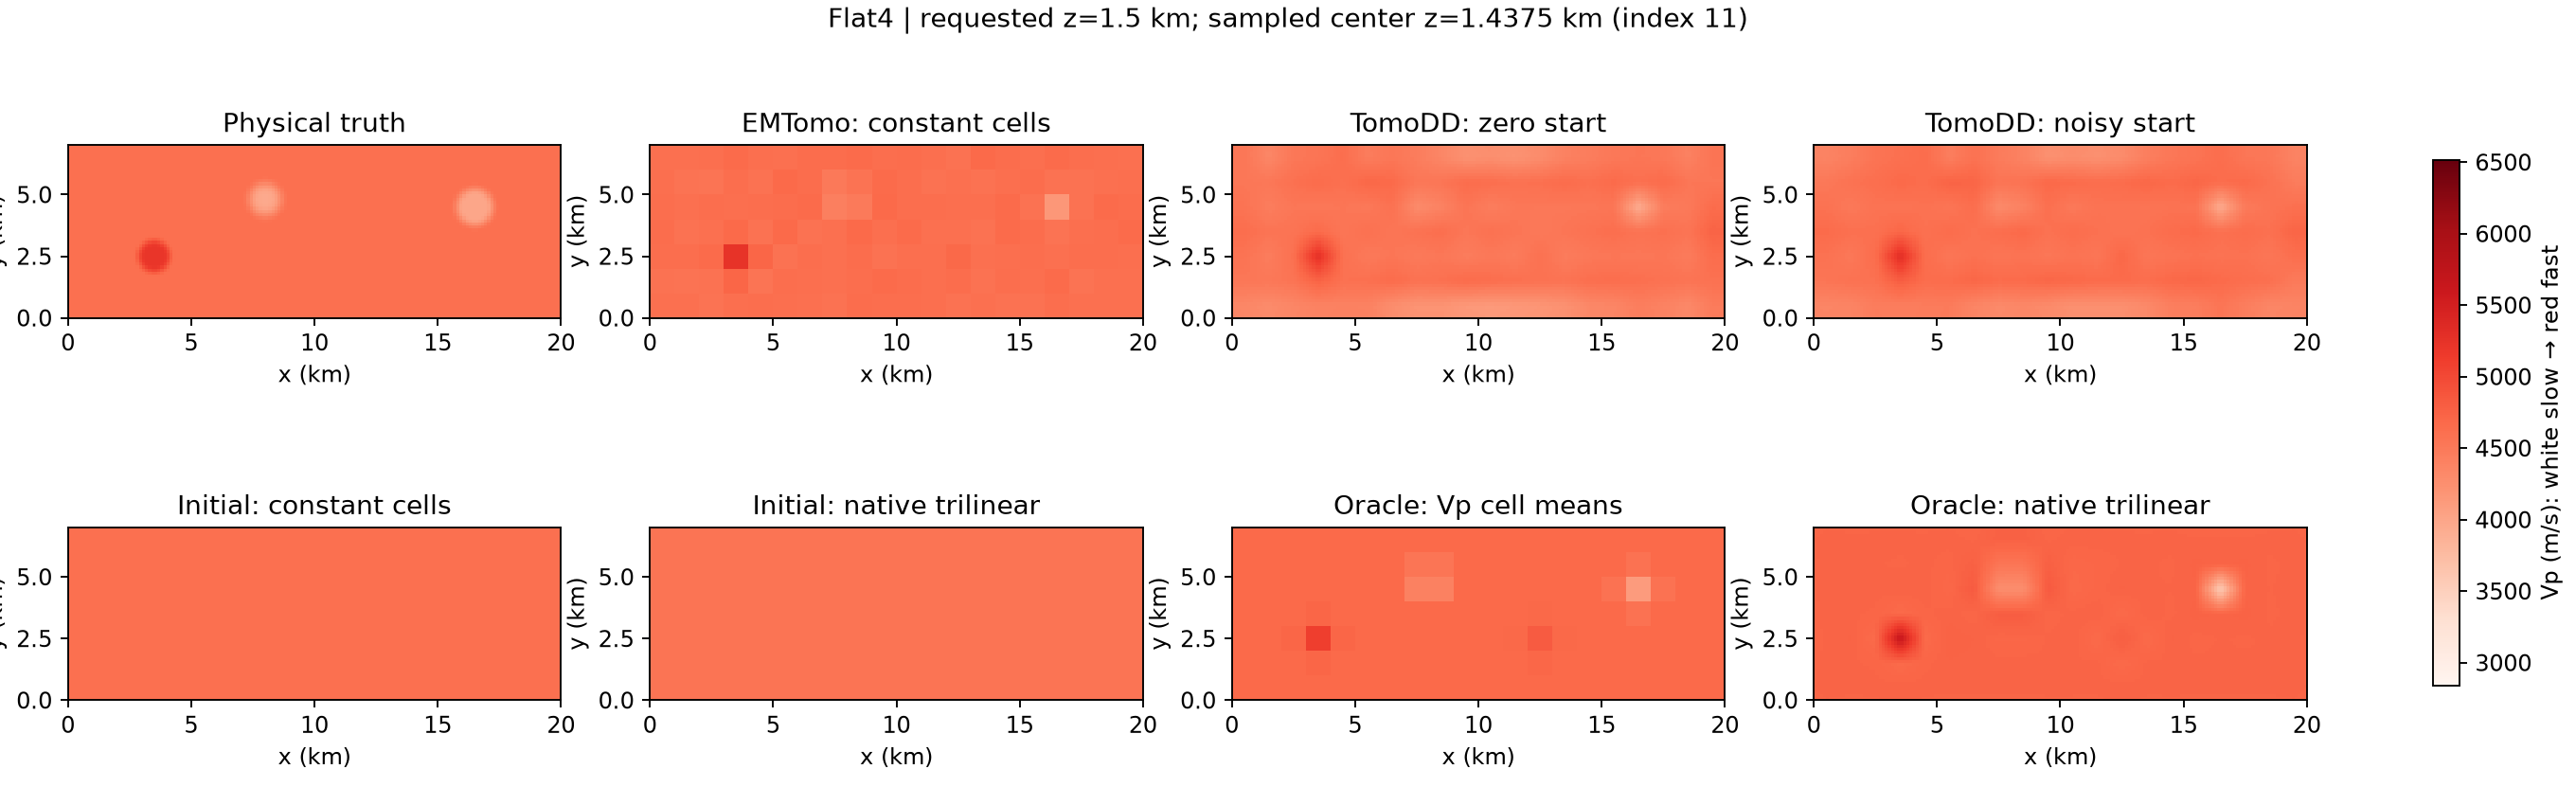
\includegraphics[width=\textwidth]{figures/flat4_synthetic_z1p4375km.png}
\caption{Layered model with artificial geometry, at the sampled truth-cell depth $z=1.4375$~km (requested plane: 1.5~km). Initial models contain no spheres; their native interpolation and their representation oracles differ. No display smoothing is added.}
\label{fig:flat4_synthetic}
\end{figure}

The available EMTomo E-step locations have 147.74-m RMS error, compared with 258.58 and 222.08~m for the two selected tomoDD catalogs (Table~\ref{tab:flat4_locations}). The noisy tomoDD start has 852.30-m initial RMS; the zero start initially has exactly zero location error. Thus relocation accuracy and velocity accuracy need not rank the workflows in the same order.

\begin{table}[tbp]
\centering
\caption{Full-catalog location errors (m). EMTomo locations are from the E-step preceding the last scored velocity update, not a relocation in the post-update model. TomoDD catalogs are from iteration three.}
\label{tab:flat4_locations}
\small
\begin{tabular}{llrrr}
\toprule
Geometry & Catalog & 3D RMS & Median & P95 \\
\midrule
Artificial & EMTomo hard & 147.74 & 107.78 & 264.59 \\
 & tomoDD, zero start & 258.58 & 216.65 & 456.58 \\
 & tomoDD, noisy start & 222.08 & 184.18 & 394.76 \\
\midrule
Geysers & EMTomo hard & 145.96 & 113.78 & 262.06 \\
 & tomoDD, zero start & 141.90 & 106.11 & 255.23 \\
 & tomoDD, noisy start & 180.58 & 123.33 & 359.83 \\
\bottomrule
\end{tabular}
\end{table}

\subsection{Same velocity model with the 2011 Geysers geometry}
\label{subsec:geysers_results}

The third series changes the acquisition geometry while keeping the velocity truth, inversion grids, and pick-noise model fixed. It uses 3776 catalog event locations from 1--20 April 2011 and 26 Geysers station positions; all arrival times remain synthetic. The model top is placed at elevation 1166~m, giving station depths 0--839~m and event depths 1.166--6.877~km. Four events outside the transformed domain are omitted. Station elevations and catalog depths are assumed to share a vertical datum, which has not been independently verified; no terrain or air layer is modeled.

EMTomo hard uses one candidate per event, 12 updates, damping one, and coverage-damping exponent two; other grid and step settings match the artificial-geometry test. TomoDD retains the same three-iteration protocol and zero/0.5-km initial-location perturbations. Whole-volume RMSE is 208.32~m/s for EMTomo and 188.75/214.69~m/s for zero/noisy-start tomoDD. Both tomoDD runs again improve sphere RMSE relative to initialization but worsen volume RMSE relative to their own initial trilinear field. The zero-start tomoDD and EMTomo location RMS values are close (141.90 and 145.96~m); the noisy-start tomoDD value is 180.58~m, from 868.86~m initially. Figure~\ref{fig:flat4_geysers} uses the same section and scale as Figure~\ref{fig:flat4_synthetic}.

\begin{figure}[tbp]
\centering
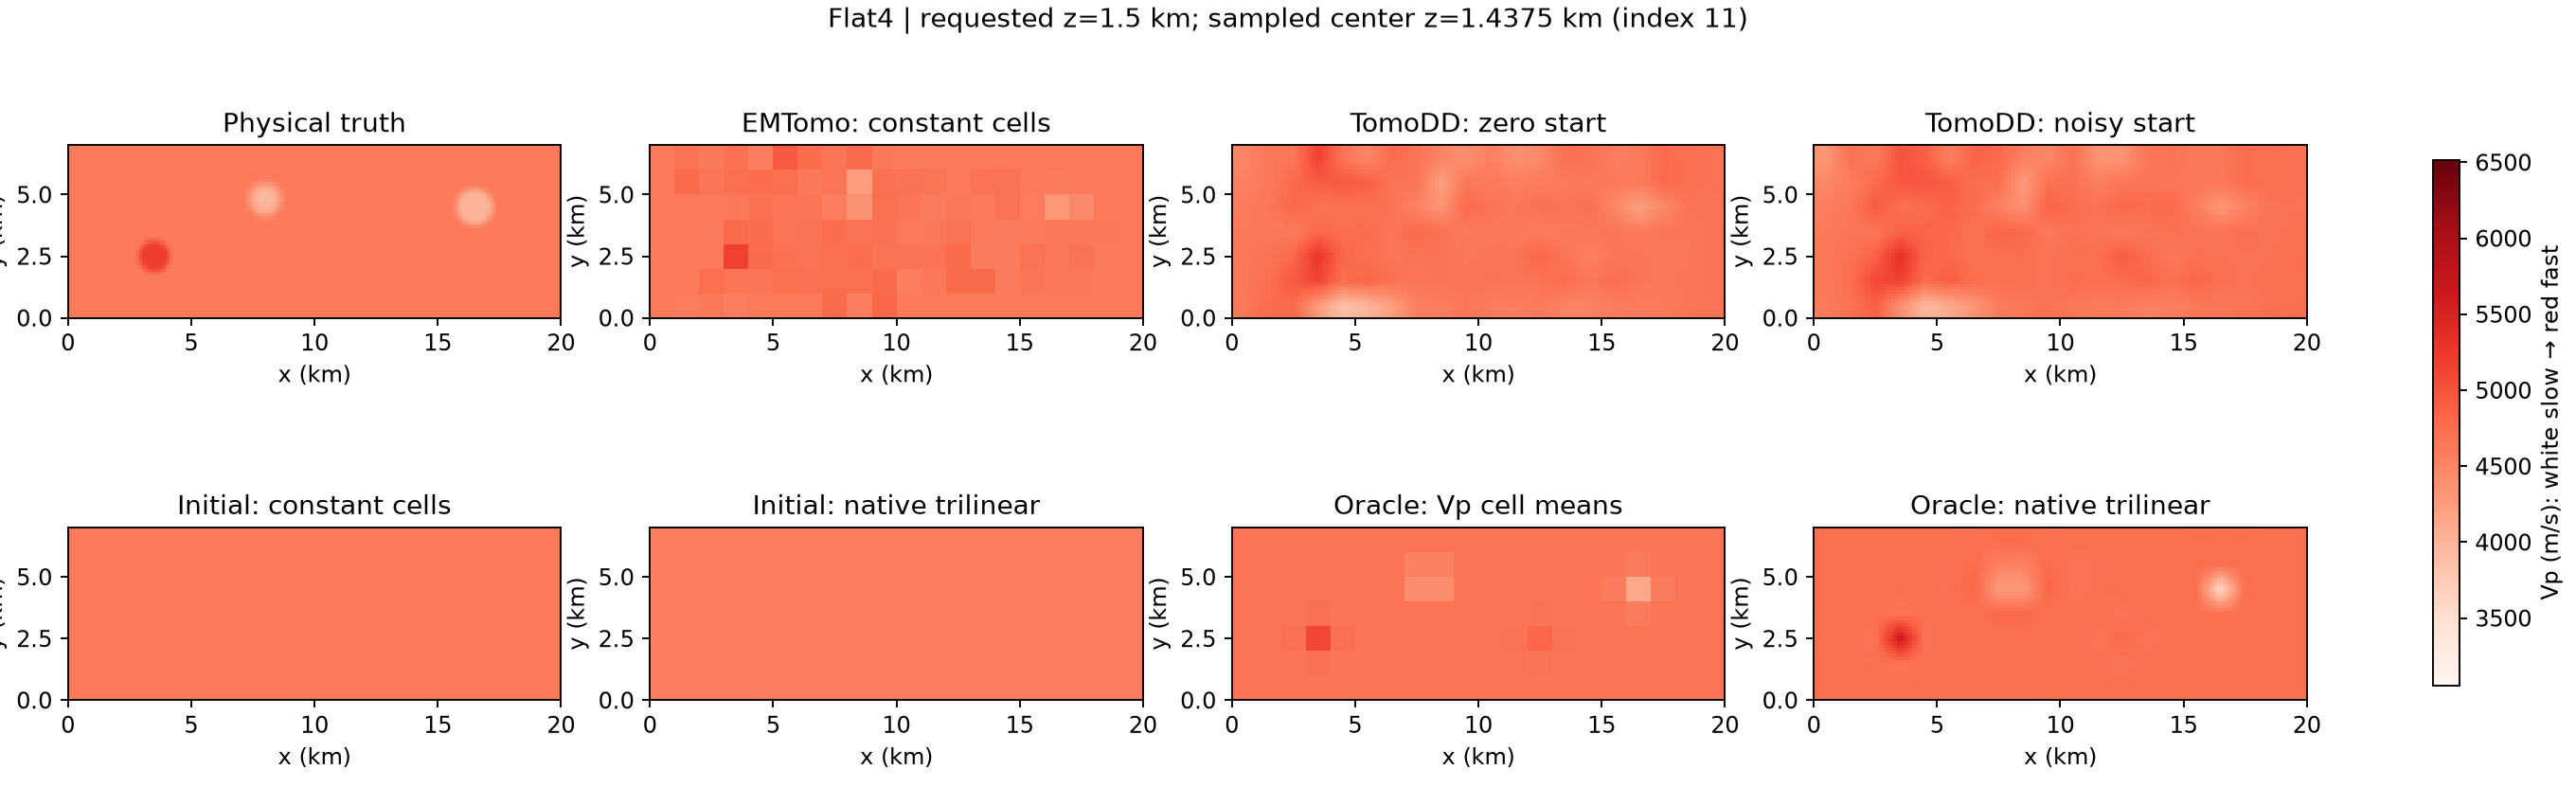
\includegraphics[width=\textwidth]{figures/flat4_geysers_z1p4375km.png}
\caption{The same layered truth and $z=1.4375$~km section as Figure~\ref{fig:flat4_synthetic}, with Geysers event--station geometry. These are reconstructions from synthetic picks, not an inversion of observed Geysers arrivals.}
\label{fig:flat4_geysers}
\end{figure}

Template amplitudes (Table~\ref{tab:sphere_amplitudes}) show that aggregate sphere RMSE does not describe every recovered anomaly. For example, EMTomo's amplitude for sphere three is 0.746 with artificial geometry and 0.827 with Geysers geometry, whereas sphere six reaches only 0.323 and 0.271. The native cell-mean oracle itself yields amplitudes below one, so under-recovered contrast is partly a representation effect. A reconstruction can exceed an oracle's individual template amplitude without improving its whole-volume error.

\begin{table}[tbp]
\centering
\caption{Signed sphere-template amplitudes $a_k$ from Eq.~\eqref{eq:sphere_amplitude}. One denotes the true template amplitude. Both oracles are fitted over the whole volume, not separately to maximize each sphere's contrast.}
\label{tab:sphere_amplitudes}
\small
\setlength{\tabcolsep}{4pt}
\begin{tabular}{lrrrrrr}
\toprule
Model & $a_1$ & $a_2$ & $a_3$ & $a_4$ & $a_5$ & $a_6$ \\
\midrule
Artificial: EMTomo hard & .439 & .617 & .746 & .784 & .525 & .323 \\
Artificial: tomoDD zero & .174 & .610 & .768 & .815 & .780 & .305 \\
Artificial: tomoDD noisy & .346 & .551 & .840 & .722 & .817 & .281 \\
Geysers: EMTomo hard & .443 & .533 & .827 & .547 & .602 & .271 \\
Geysers: tomoDD zero & .516 & .448 & .834 & .476 & .958 & .428 \\
Geysers: tomoDD noisy & .652 & .373 & .870 & .341 & .956 & .508 \\
\midrule
Constant-cell oracle & .485 & .503 & .677 & .753 & .497 & .463 \\
Trilinear oracle & .666 & .677 & .908 & .862 & .741 & .627 \\
\bottomrule
\end{tabular}
\end{table}

\subsubsection{Soft-assignment sensitivity}

Separate completed Geysers runs retain $K=5,10,15$ hypotheses at temperature one. They share the hard run's input hashes, initial velocity field, regularization, and 12-update endpoint. However, both the shortlist size and retained-hypothesis count change with $K$; comparison with hard $K=1$ is not an isolated test of soft versus hard weights. Table~\ref{tab:soft_geysers} reports every available $K$, without selecting the best result post hoc.

\begin{table}[tbp]
\centering
\caption{Geysers candidate-count sensitivity. Velocity errors are in m/s; all location quantities are in m. Location scores use the preceding E-step for every run.}
\label{tab:soft_geysers}
\small
\begin{tabular}{lrrrrr}
\toprule
Assignment & Volume RMSE & Sphere RMSE & MAP RMS & Mean ES & RMS spread \\
\midrule
Hard, $K=1$ & 208.32 & 329.69 & 145.96 & 127.68 & 0.00 \\
Soft, $K=5$ & 208.27 & 330.13 & 140.12 & 103.36 & 55.72 \\
Soft, $K=10$ & 208.26 & 330.20 & 138.30 & 95.38 & 80.31 \\
Soft, $K=15$ & 208.29 & 330.18 & 138.65 & 93.24 & 94.32 \\
\bottomrule
\end{tabular}
\end{table}

The available soft runs have lower mean energy scores and slightly lower mode-location RMS, but essentially unchanged volume velocity RMSE and slightly higher sphere RMSE. Increasing the number of retained hypotheses therefore does not produce an appreciable velocity-reconstruction gain in this example. RMS spread in the table is the catalog root-mean weighted squared distance about each event's weighted mean, not a calibrated confidence radius.

\todo{Verify the legacy checkerboard runtime implementation or repeat the series with the current implementation; complete the matched soft/hard experiment for artificial geometry; extract checkerboard EMTomo location scores; perform final location-only passes to synchronize EMTomo velocity and location checkpoints. For a clean weight-treatment ablation, keep the same candidate shortlist in hard and soft runs. Confirm the Geysers catalog/station vertical datum and document checkpoint-selection rationale and runtimes before submission.}
